\section{Introduction}
\label{sec:intro}

\subsection{Context and motivation}

Ant scans can turn specimens that are difficult to measure repeatedly into a
source of comparable three-dimensional traits. If every scan is registered to
a common parametric model, quantities such as head width, Weber's length or
appendage proportions can be extracted systematically instead of by hand under
a microscope, which opens a route to studying biodiversity at population
scale. Real scans, whether from scAnt photogrammetry~\cite{scant} or
micro-CT, are far from ideal inputs: they contain holes, self-intersections,
arbitrary orientation and missing surface exactly at the thin structures of
greatest anatomical interest (Figure~\ref{fig:raw-scans}).

\begin{figure}[!htb]
\centering
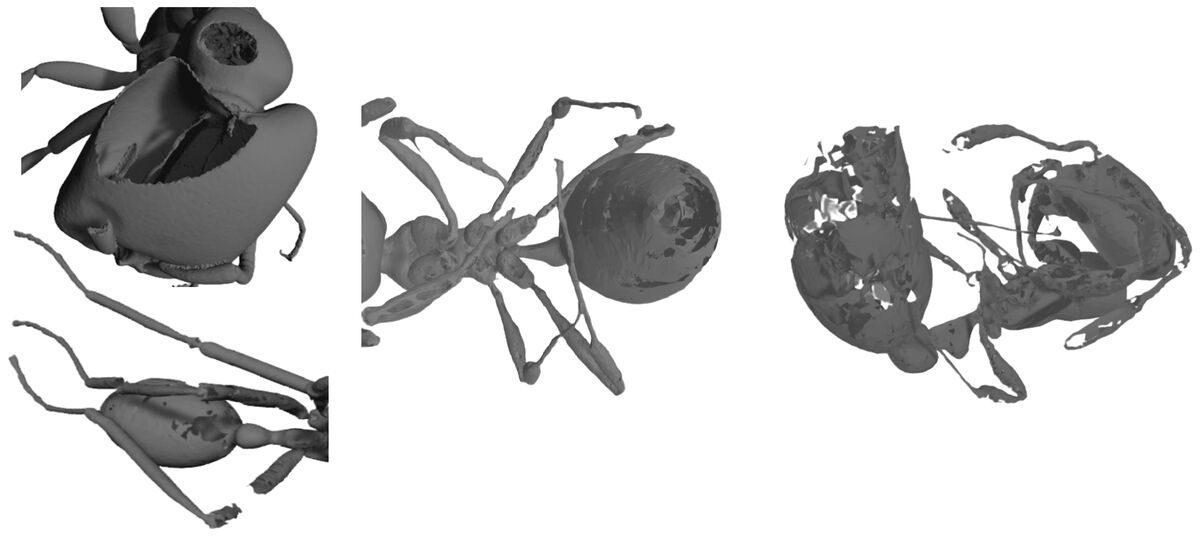
\includegraphics[width=0.62\linewidth]{figures/fig_before_registration.jpg}
\caption[Raw scans before registration]{Raw scans before registration: holes,
self-intersections and missing surface at the structures of greatest
anatomical interest.}
\label{fig:raw-scans}
\end{figure}

The method studied here, SMILify, builds on SMALify~\cite{smalify}, an
optimisation-based framework for fitting the SMAL quadruped model~\cite{smal}.
Its ambition is to turn any rigged mesh into a SMAL-compatible parametric
model, with SMIL (Skinned Multi-Insect Linear) as the current insect-focused
instance. At the start of the internship, of roughly 380 raw scans in the
available corpus only 86 (about 23\%) had been curated as clean enough for
registration.

In the first week of July 2026, ten preprocessed ant scans were passed through
the registration pipeline. All ten optimisations converged cleanly: no
divergence, and a numerical objective that decreased as expected. Yet four of
the resulting models were not recognisable as ants. Legs had collapsed into
the gaster and, in some fits, the head had been absorbed into the thorax.
Several of these anatomically wrong fits even reached a \emph{lower} loss
than the runs that had visibly succeeded. The optimiser had succeeded; the
registration had failed. This discrepancy is the starting point of the
internship. The objective is a symmetric point-to-point distance between two
surfaces: it measures whether the fitted mesh \emph{covers} the target, not
whether vertex $i$ of the template has landed on the anatomical point it is
defined to represent. When the two diverge, nothing in the pipeline's own
numerical output signals it.

\subsection{Problem statement and research questions}
\label{sec:problem}

Registration recovers, for a scan $T$, the latent variables of a parametric
mesh $M$ with shape $\bm\beta$, articulated pose $\bm\theta$, scale $s$ and
residual per-vertex deformation $\mathbf d$:
\begin{equation}
(\hat{\bm\beta},\hat{\bm\theta},\hat s,\hat{\mathbf d})
 =\arg\min_{\bm\beta,\bm\theta,s,\mathbf d}\;
 \mathcal{L}\big(M(\bm\beta,\bm\theta,s,\mathbf d),\,T\big).
\label{eq:registration}
\end{equation}
The scan is only a set of surface samples: it carries no vertex identities, no
joint locations and no anatomical labels, yet these are exactly the
quantities to be recovered. Equation~\eqref{eq:registration} is non-convex and
its objective observes surfaces only, so several different latent
configurations can produce nearly the same surface. The mapping from observed
surface to anatomical state is therefore not guaranteed to be identifiable.
Every mechanism studied in this report is a symptom of that one ambiguity.
Four research questions structure the work:
\begin{enumerate}[label=\textbf{RQ\arabic*.}]
\item Is input mesh quality the dominant limit on registration accuracy?
\item Does a good surface fit imply a correct anatomical fit?
\item Which component (initialisation, sampling, deformation freedom,
correspondence or the objective) limits anatomical recovery, and where along
the body?
\item When a parameter is recovered, when is it a valid biological
measurement?
\end{enumerate}

\subsection{Objectives of the internship and contribution}

The internship brief listed six assignments: unify the preprocessing pipeline,
stabilise a Shape-Diameter-Function-based segmentation, integrate neural
initialisation, design a hybrid registration framework, benchmark the result
and deliver documentation. Together they imply a hypothesis, namely that input
mesh quality is the limiting factor. An early, controlled test of that
hypothesis was negative (\F{F2}), and the work was redirected, with my
supervisor, toward initialisation, sampling, anatomical structure,
correspondence and finally the objective itself.

SMILify already provided the parametric representation and a baseline fitting
pipeline. My contribution is the diagnostic and validation machinery built
around it and what that machinery established: a synthetic round-trip
correspondence benchmark, a three-level evaluation protocol, counterfactual
(oracle) interventions, a corrected and frozen expert benchmark, and several
algorithmic and systems extensions, each judged against a criterion fixed
before the experiment (Table~\ref{tab:contrib}). The central result is that
surface fit, anatomical correspondence, parameter recovery and measurement
validity are four distinct properties that do not track one another.

\subsection{Structure of the report}

Section~\ref{sec:host} presents the host organisation: its domain of activity,
its structure and the professions present. Section~\ref{sec:work} describes and
analyses my work and its place in the institute: the technical framework, the
methodology, the diagnosis of the registration bottleneck, the interventions
tested and the step from registration to measurement. Section~\ref{sec:conclusion}
concludes with limitations, outlook and what the internship taught me.
